\chapter{Monitoraggio e controllo}
\label{ch:monitoraggio-e-controllo}

Il progetto è stato gestito col supporto di \emph{GitHub Projects}~\cite{cit:github-projects}. Questo strumento si integra con il DVCS Git utilizzato dal team e permette di gestire le attività di sviluppo in modo agile.
Inoltre, è stata prestata grande attenzione ad automatizzare il più possibile queste attività per ridurre al minimo il tempo necessario per la loro esecuzione e permettere agli sviluppatori di concentrarsi sui problemi di business.

\section{Reporting automatico}
\label{sec:reporting-automatico}

Ogni task dello sprint viene convertito in una GitHub issue~\cite{cit:github-issues} che ne riporta le dipendenze e le informazioni di base; un esempio di tale issue è riportato in \Cref{fig:issue-example}. Come mostrato in figura, il vantaggio di tale approccio sta nella possibilità di automatizzare il reporting delle attività svolte durante lo sprint. Infatti, un bot può analizzare le dipendenze fra task -- ricostruendo così lo sprint network diagram --, calcolare il percorso critico e notificare gli sviluppatori di eventuali ritardi.

Grazie alla stretta integrazione fra il sistema di reporting e il DVCS, il programmatore non dovrà occuparsi di gestire alcun overhead dato che gli sarà sufficiente chiudere una issue per segnalare che il task corrispondente è stato completato.

\begin{figure}[htp]
  \centering
  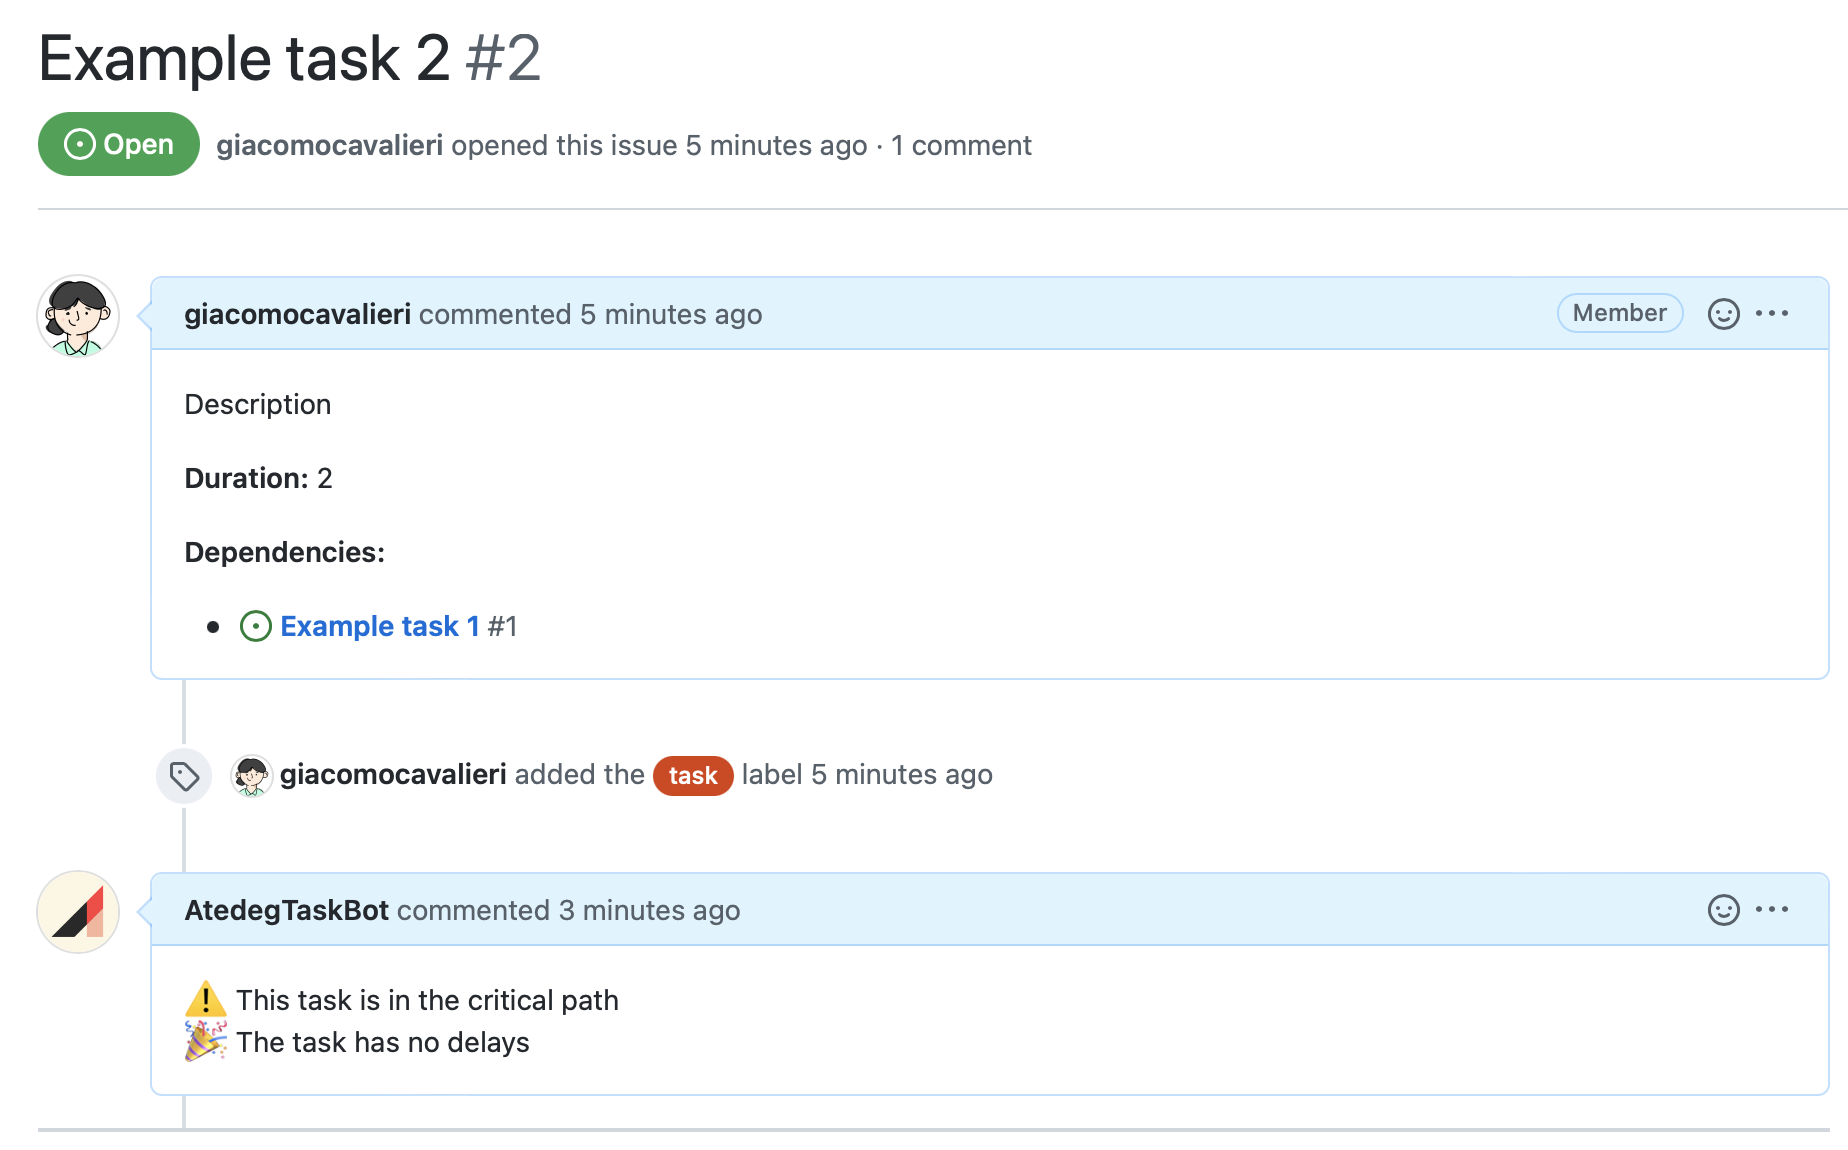
\includegraphics[width=\textwidth]{images/task-example.png}
  \caption{Esempio di issue}
  \label{fig:issue-example}
\end{figure}

\subsection{Sprint burndown chart}
Inoltre, ad ogni sprint viene generato automaticamente uno \emph{sprint burndown chart} a partire dalle issue chiuse. Questo grafico viene aggiornato al completamento dei task e permette di monitorare lo stato di avanzamento dello sprint in tempo reale.
È uno strumento fondamentale che permette di individuare rapidamente dei ritardi sulla tabella di marcia permettendo al team di analizzarne le cause tempestivamente.

Come mostrato in \Cref{fig:sprint-burndown-chart}, il grafico riporta sull'asse delle ascisse il giorno dello sprint e sull'asse delle ordinate l'effort rimanente. Inflessioni del grafico indicano ritardi o avanzamenti rispetto alla tabella di marcia ideale.

\begin{figure}
\centering
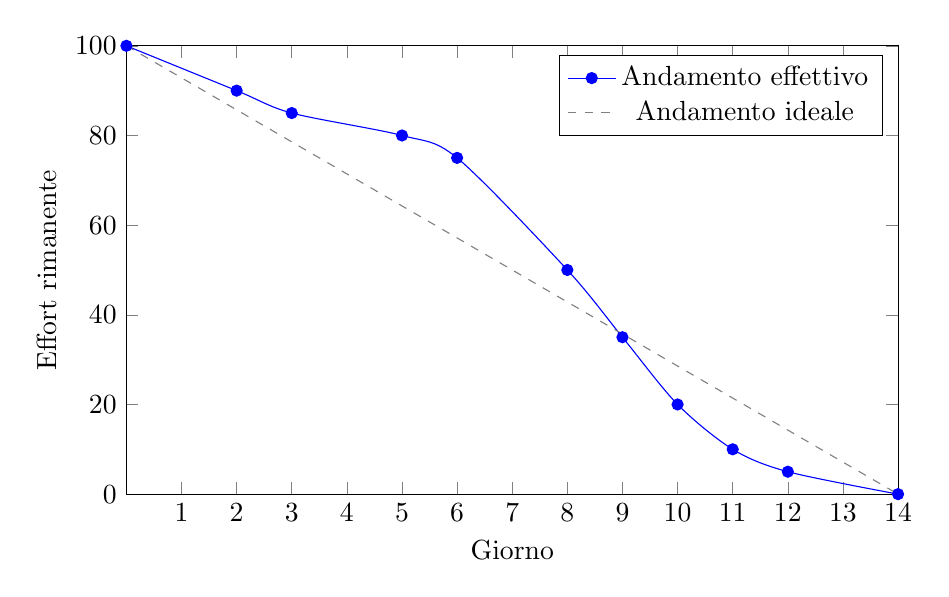
\begin{tikzpicture}
  \begin{axis}[
      xlabel={Giorno},
      ylabel={Effort rimanente},
      xmin=0, xmax=14,
      x=0.7cm,
      ymin=0, ymax=100,
      xtick={1,...,14},
      ytick={0,20,...,100}]
  \addplot[smooth,mark=*,blue] plot coordinates {
      (0,100)
      (2,90)
      (3,85)
      (5,80)
      (6,75)
      (8,50)
      (9,35)
      (10,20)
      (11,10)
      (12,5)
      (14,0)
  };
  \addlegendentry{Andamento effettivo}
  
  \addplot[dashed,color=gray,mark=none]
      plot coordinates {
          (0,100)
          (14,0)
      };
  \addlegendentry{Andamento ideale}
  \end{axis}
\end{tikzpicture}
\caption{Esempio di sprint burndown chart}
\label{fig:sprint-burndown-chart}
\end{figure}

\subsection{Project Burndown Chart}
È stato anche realizzato un \emph{project burndown chart} che mostra lo stato di avanzamento del progetto. 
Anche in questo caso il grafico viene generato automaticamente a partire dalle issue chiuse e permette di monitorare l'intero progetto.
Come mostrato in \Cref{fig:project-burndown-chart}, il grafico riporta gli sprint sull'asse delle ascisse e il numero di story point rimanenti sull'asse delle ordinate.

Questo strumento è fondamentale per poter stimare la velocità di sviluppo del team nel consumare story points. Infatti, per stimare il numero di story points da realizzare in uno sprint devono essere tenute in considerazione le storie concluse in precedenza ed eventuali difficoltà del team nel portarle a compimento.
Così facendo è possibile mantenere una velocità di sviluppo all'incirca costante per poter stimare con maggior precisione le tempistiche di consegna del progetto.

\begin{figure}
  \centering
  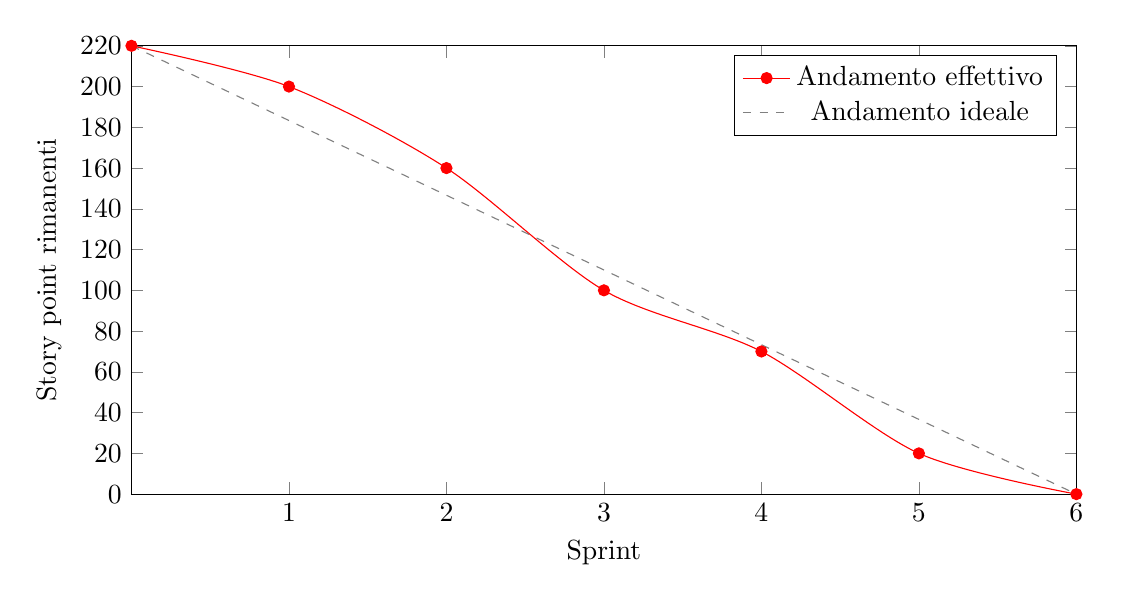
\begin{tikzpicture}
    \begin{axis}[
        xlabel={Sprint},
        ylabel={Story point rimanenti},
        xmin=0, xmax=6,
        x=2cm,
        ymin=0, ymax=220,
        xtick={1,...,6},
        ytick={0,20,...,220}]
    \addplot[smooth,mark=*,red] plot coordinates {
        (0,220)
        (1,200)
        (2,160)
        (3,100)
        (4,70)
        (5,20)
        (6,0)
    };
    \addlegendentry{Andamento effettivo}
    
    \addplot[dashed,color=gray,mark=none]
        plot coordinates {
            (0,220)
            (6,0)
        };
    \addlegendentry{Andamento ideale}
    \end{axis}
  \end{tikzpicture}
  \caption{Esempio di project burndown chart}
  \label{fig:project-burndown-chart}
  \end{figure}

